\documentclass[11pt,titlepage,dvipdfmx,twoside]{article}
\linespread{1.1}

\usepackage{amsfonts}
\usepackage{amssymb}
\usepackage{amsmath}
\usepackage{amsthm}
\newtheorem{theorem}{Theorem}
\newtheorem{lemma}[theorem]{Lemma}
\usepackage{enumitem}
\usepackage{geometry}
\geometry{a4paper, left=2.5cm,right=2.5cm,top=2.5cm,bottom=2.5cm}

\usepackage{algorithm}  
\usepackage{algorithmic}  
\renewcommand{\algorithmicrequire}{\textbf{Input:}} 
\renewcommand{\algorithmicensure}{\textbf{Output:}}
\renewcommand{\algorithmicforall}{\textbf{for each}}

\usepackage{mathtools}
\usepackage{comment}
\usepackage[dvipdfmx]{graphicx}
\usepackage{float}
\usepackage{framed}
\usepackage{graphicx}
\usepackage{subcaption}
\usepackage{listings}
\usepackage{plistings}
\usepackage{color}
\usepackage{url}
 
\definecolor{codegreen}{rgb}{0,0.6,0}
\definecolor{codegray}{rgb}{0.5,0.5,0.5}
\definecolor{codepurple}{rgb}{0.58,0,0.82}
\definecolor{backcolour}{rgb}{0.95,0.95,0.92}
 
\lstdefinestyle{mystyle}{
    %backgroundcolor=\color{backcolour},   
    frame=single,
    commentstyle=\color{codegreen},
    keywordstyle=\color{magenta},
    numberstyle=\tiny\color{codegray},
    stringstyle=\color{codepurple},
    basicstyle=\footnotesize,
    breakatwhitespace=false,         
    breaklines=true,                 
    captionpos=b,                    
    keepspaces=true,                 
    numbers=left,                    
    numbersep=5pt,                  
    showspaces=false,                
    showstringspaces=false,
    showtabs=false,                  
    tabsize=2
}
\renewcommand{\lstlistingname}{Code sample}
\lstset{style=mystyle}

\title{\Huge{
Using Python and Scikit-learn to Construct Artificial Neural Networks}}

\begin{document}

% The following makeatletter must be after begin{document}
\makeatletter 
\let\c@lstlisting\c@figure
\makeatother

\date{\today}

\maketitle

% \cleardoublepage

\thispagestyle{empty}
\tableofcontents
\clearpage

\pagenumbering{arabic}

\section{Outline}
In this text we explain how to construct an artificial neural network that 
given known data of chemical compounds and their properties,
will predict the property of an unknown chemical compound.
For this purpose, chemical compounds are represented as 
{\em feature vectors} that are obtained from the structure of the compounds.
We will describe a program that given pairs of feature vectors of chemical compounds
and values for some chemical property, constructs an artificial neural network,
and explain how to get the parameters (weights and biases) of the trained neural network.

We use the scikit-learn library for machine learning in the Python programming language.
Please check further details at the following web-page:
\url|https://scikit-learn.org/stable/|

\smallskip
Note that this text is accompanied by the following three files

\begin{itemize}
\item {\tt scikit\_chemgraph\_learning.py}\\
A program written in Python that 
given a dataset of pairs of feature vectors and observed values of chemical properties,
constructs an artificial neural network using 5-fold cross-validation.
The weights and biases of the trained neural network that achieved 
the highest coefficient of determination (${\rm R}^2$) score over the test data are stored as output files.
Further details are given in Section~\ref{sec:section4}.

\item {\tt ha\_fv4\_plus.csv} \\
Computed feature vectors of chemical compounds in
the PubChem database with known values for the property \emph{heat of atomization}.

\item {\tt ha\_target\_data.csv}\\
A comma-separated-value file containing observed values 
of chemical property {heat of atomization}
of compounds in the PubChem chemical database.
 
 \medskip 
Section~\ref{sec:section3} contains further details on the file format, and
Section~\ref{sec:section5} gives the results of computational experiments
using the dataset from the above two files.
\end{itemize}


The remainder of this text is organized as follows. 
Section~\ref{sec:section2} gives basic terminology used throughout the text.
Section~\ref{sec:section3} explains the format of the input and output of the program.
In particular, an actual example of program input and output is used.
Section~\ref{sec:section4} gives further details on the source code of the program.
Section~\ref{sec:section5} gives the results of an actual computational experiment.

\newpage

\section{Terminology}
\label{sec:section2}

In this section we explain some of the terminology used throughout the text. 


\begin{itemize}
\item Feature vector\\
A vector of numerical values describing a chemical compound, such as the number of
atoms of each element type, or 
calculated based on the topology of the graph representation
of a chemical compound, such as the graph's diameter.

\item Neural network \\
Artificial neural networks, or simply neural networks, 
are one of the most well-established methods in machine learning.
They are used to predict a value based on an input vector.
In this text, the input to neural networks is a feature vector of a chemical compound,
and the output is a predicted value for a certain chemical property.

\item Input layer, hidden layers, output layer \\
We assume the multi-layer perceptron model for artificial neural networks.
In this model, neural networks comprise several {\em layers}.
The first of these layers is the input layer, taking numerical data,
in out case, from a feature vector, and therefore the input layer
has the same number of nodes as elements in the feature vector.
Next, these numeric values are propagated through
the networks {\em hidden} layers, where the calculation of
one layer is used as an input to the next.
At last, the output layer gives the predicted value based on the 
input vector.

\item Weight\\
In a neural network nodes are interconnected by edges, and each edge is assigned a 
numerical value, or {\em weight}.
The propagation of the values from the input layer to the output layer
involves calculation based on these weights.

\item  Bias \\
Each node in the hidden layers of a neural network is
assigned a numerical value, called a {\em bias},
which together with the weights is used in 
calculating an output value based on the input vector.
\medskip

The neural network ``learns'' by calculating a set of weights and biases
based on given pairs of input vectors and target values.

\item Activation function\\
 An activation function is assigned to each node of a neural network, and is used 
 in calculating an output value from a given vector of input values.
 In particular, the output value of each node is the value of the activation function given
 as input a linear combination of the outputs of the nodes from the previous layer, weighted by
 the corresponding edge weights.


\end{itemize}

\newpage

\section{Program Input and Output}
\label{sec:section3}

This section gives details on the input and output format of the Python program.
Section~\ref{sec:section3_1} gives an explanation of the input to the program using 
an actual example with the chemical property heat of atomization.
Section~\ref{sec:section3_2} gives details of the input data format.
Section~\ref{sec:section3_3} gives an explanation of the actual output produced from the input data.
Section~\ref{sec:section3_4} explains the format of the output data.

\subsection{Program Input}
\label{sec:section3_1}

As input the Python program takes two sets of data.
One is a file containing the feature vectors of a set of chemical compounds, 
and the other is a file containing the numerical values of some observed chemical property
over the same set of compounds.
The program constructs and trains a neural network given these two files.

\bigskip

\subsection{Input data format}
\label{sec:section3_2}

This section describes the format of the two files that  are input
to the program as explained in Section~\ref{sec:section3_1}.

First, we explain the format of the file giving the feature vectors.
It is a comma-separated-value (csv) file, in plain text format.
The first row gives the names of each descriptor of the feature
vector, whose first entry is the a compound identification number (CID)
of the chemical compound, and is not used in learning or prediction.
Following, from the second row onward, the feature vector
of several chemical compounds are given, each value separated by a comma, 
and each feature vector in one line.

\bigskip

\begin{oframed}
{\bf Feature vector file format}(Note: \verb|\\| shows that there is NO line break.)\\\\
%\bigskip\bigskip
CID,n,M,C\_in,C\_ex,O\_in,O\_ex,S\_in,S\_ex,H,C1O\_in,C1O\_ex,C1C\_in,C1C\_ex,C2C\_in,C2C\_ex,\verb|\\| \\
C1S\_in,C1S\_ex,\ldots \\
263,5,128,1,3,0,1,0,0,10,0,1,0,3,0,0,0,0, \ldots \\
6560,5,128,2,2,0,1,0,0,10,0,1,1,2,0,0,0,0, \ldots \\
6568,5,128,2,2,0,1,0,0,10,0,1,1,2,0,0,0,0, \ldots \\
6386,5,128,1,3,0,1,0,0,10,0,1,0,3,0,0,0,0, \ldots \\
6276,6,126.667,2,3,0,1,0,0,12,0,1,1,3,0,0,0,0,\ldots \\
\hspace{5mm}\vdots
\\
\hspace{5mm}\vdots

\end{oframed}


Next we explain the structure of a csv file that contains 
the target values of a chemical property.
The first line simply gives the table heading as ``CID,a'', where CID is
a compound's ID number, and ``a'' denotes the target value.
The following lines are the ID and target values of chemical compounds, 
given in the same order as in the feature vector csv file.

\bigskip

\begin{oframed}
{\bf Target data file format (example of heat of atomization)}\\\\
%\bigskip\bigskip
CID,a \\
263,1329.95 \\
6560,1332 \\
6568,1334.14 \\
6386,1338.88 \\
6276,1609.92 \\
\hspace{5mm}\vdots
\\
\hspace{5mm}\vdots

\end{oframed}


\subsection{Program output}
\label{sec:section3_3}

Figure~\ref{fig:sample} gives an example of a trained neural network, 
with calculated edge weights and node biases.
The final output of the program is a file containing the
weights and biases of a trained neural network.


\begin{figure}[H]
  \centering
  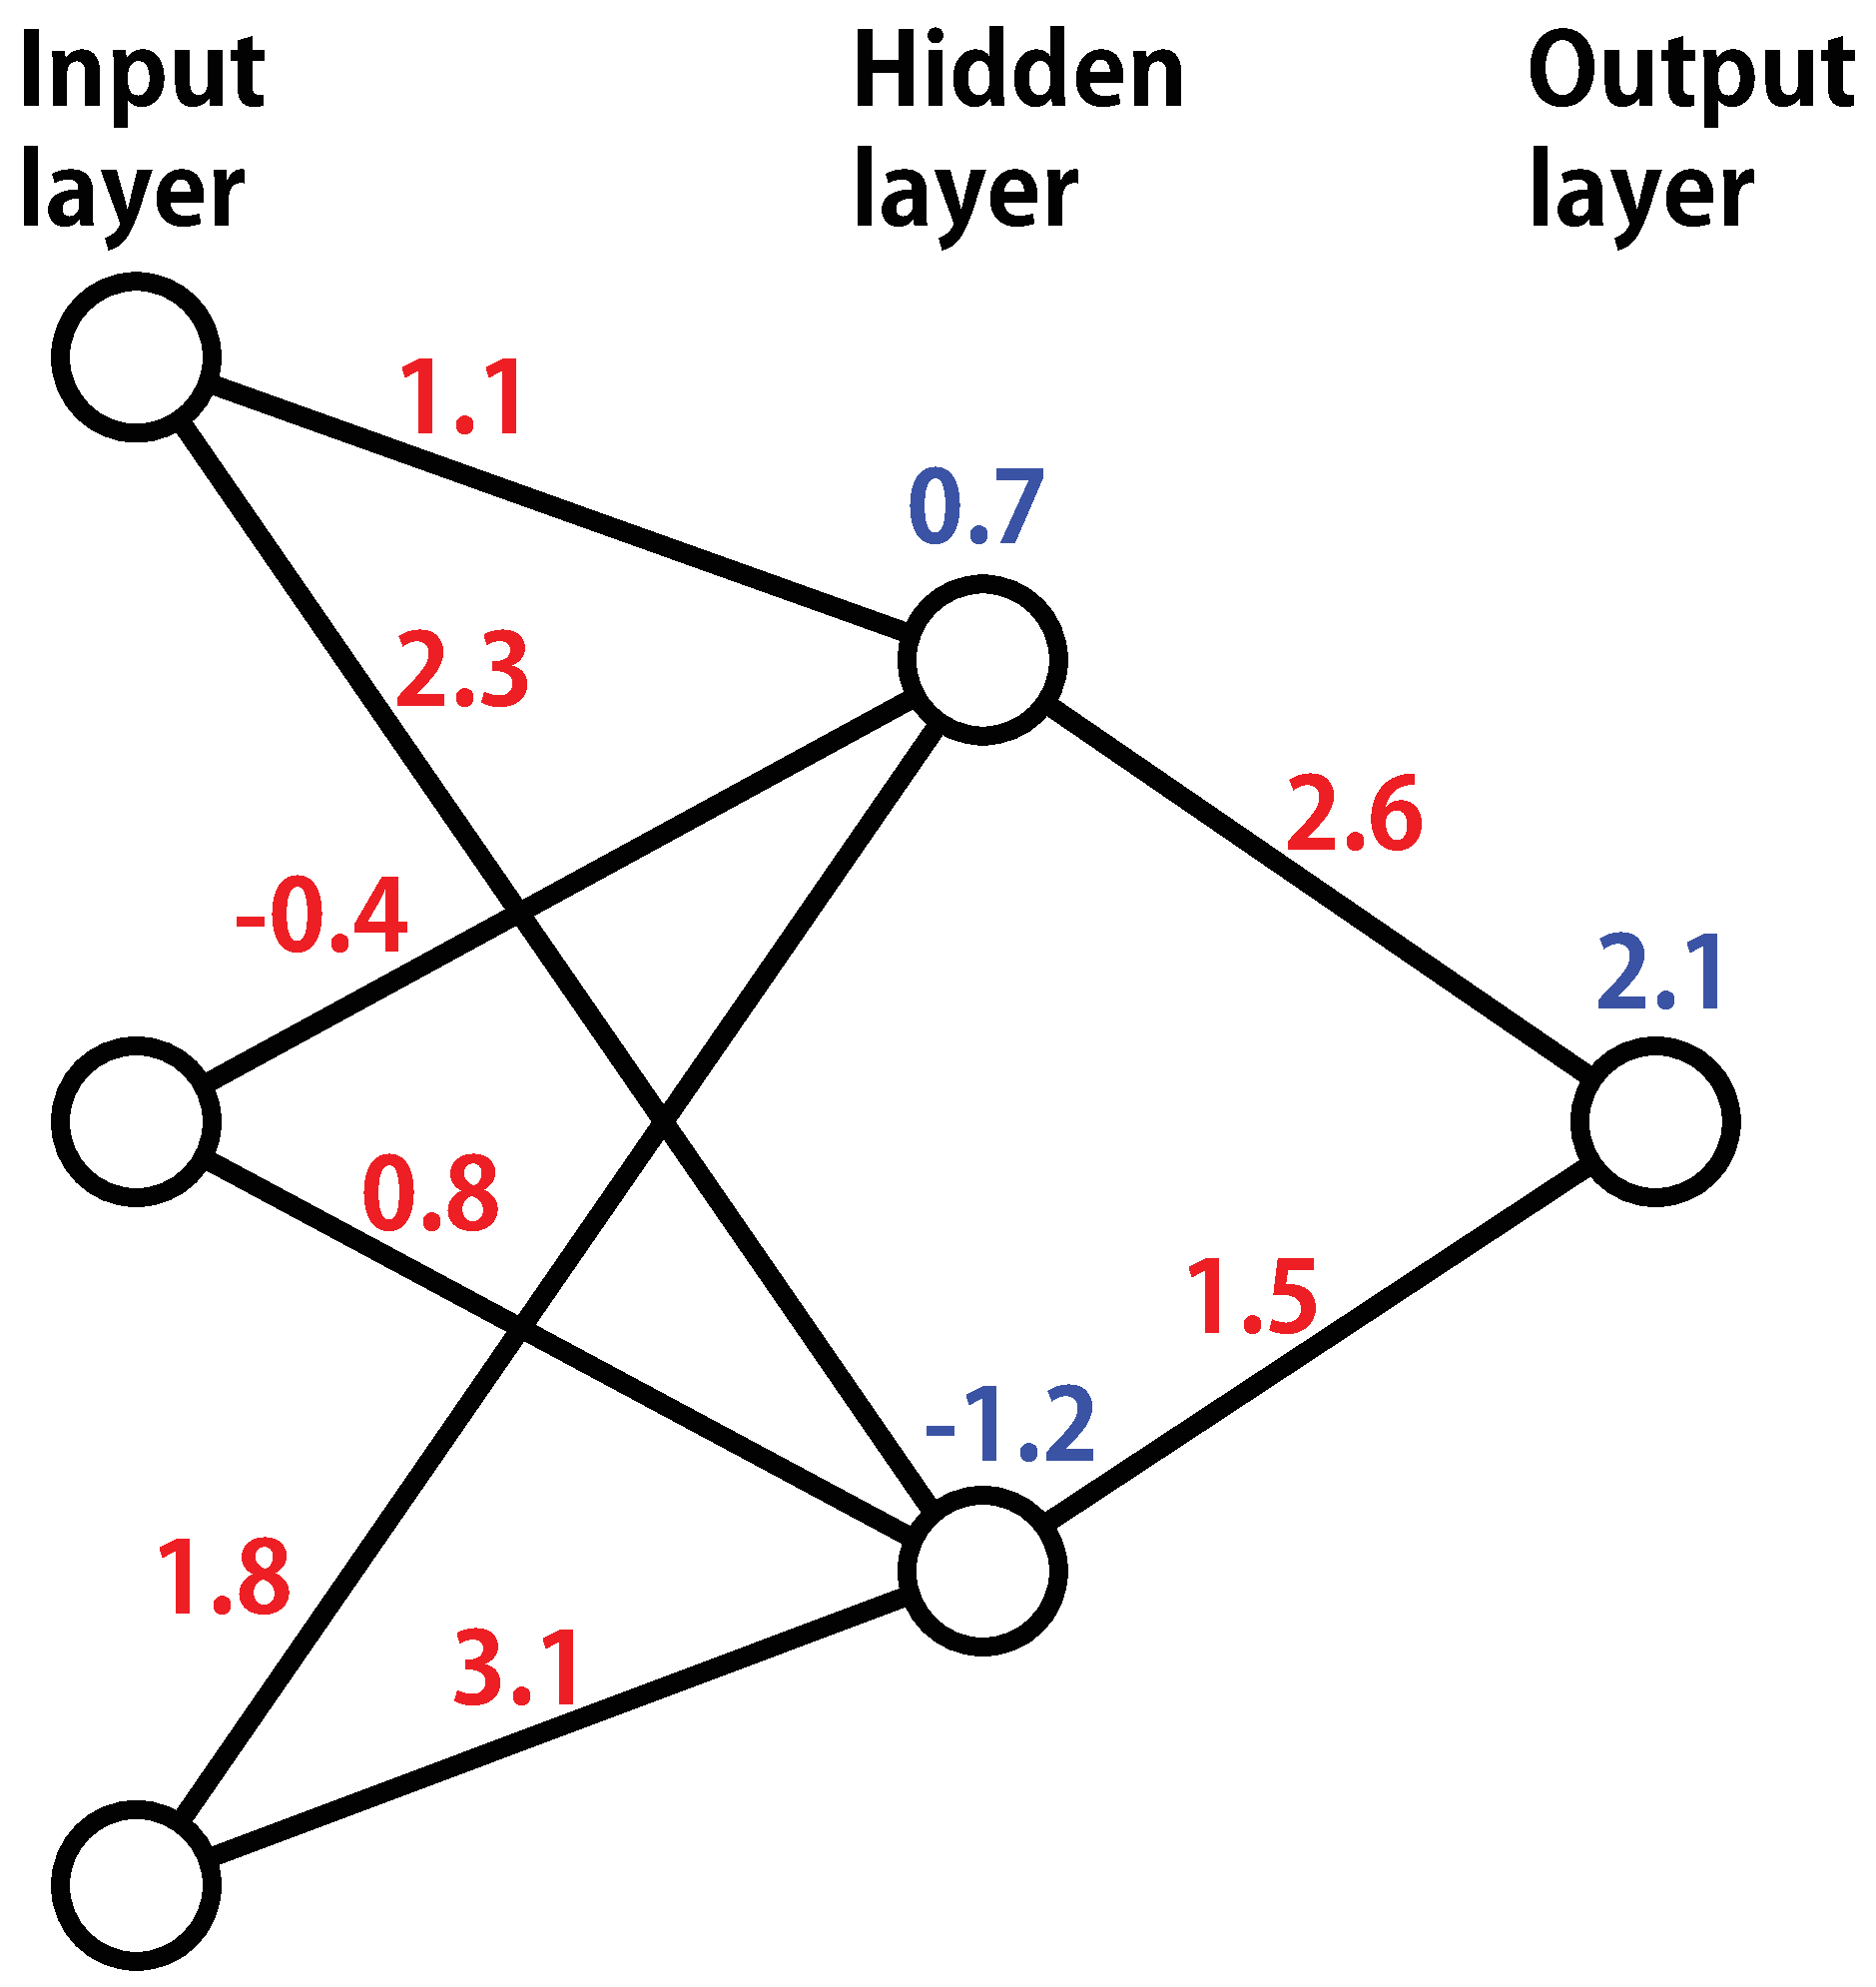
\includegraphics[width = 0.4 \textwidth]{./fig/ANN_sample_en}
  \caption{An example of a trained artificial neural network.
  The red numbers next to edges give the weights, 
  and blue numbers next to nodes give the biases.}
  \label{fig:sample}
\end{figure}


\subsection{Output format}
\label{sec:section3_4}

The edge weights and node biases resulting from a trained neural network from the
program are written in two respective output files.

The first line of the output file with edge weight data
gives the architecture of the artificial neural network,
that is, the number of nodes in the input layer, then the numbers of nodes in each hidden
layer, and finally, the number of nodes in the output layer.
From the second line onward follow the values of the edge weights.
Each row gives the values of the edges going out of a single node.

\bigskip

\begin{oframed}
{\bf Output file format, edge weights for the example in Fig.~\ref{fig:sample}}\\\\
%\bigskip\bigskip
3 2 1\\
1.1 2.3\\
-0.4 0.8\\
1.8 3.1\\
2.6\\
1.5\\
\end{oframed}

\bigskip

The file containing the node biases contains one node bias value per line.
Not that nodes in the input layer do not have bias values.

\bigskip

\begin{oframed}
{\bf Output file format, node biases for the example in Fig.~\ref{fig:sample}}\\\\
%\bigskip\bigskip
0.7\\
-1.2\\
2.1\\
\end{oframed}

\bigskip

\newpage

\section{Explanation of the program}
\label{sec:section4}

This section explains a program implemented
in the Python programming language that
reads input files with feature vector values and target data
as explained in Sections~\ref{sec:section3_1} and~\ref{sec:section3_2},
trains an artificial neural network using five-fold cross-validation,
and produces output files containing the edge weights and node biases of
the neural network that achieves the highest coefficient of determination (R$^2$)
test score over the five cross-validation tests.
The format of the output files is as described in Sections~\ref{sec:section3_3} and~\ref{sec:section3_4}.

The source code of the program is given in the file {\tt scikit\_chemgraph\_learning.py},
and given completely as code sample~\ref{code:ANN}.

\bigskip\bigskip

\begin{lstlisting}[ language=Python,label={code:ANN},
  caption={Source code file {\tt scikit\_chemgraph\_learning.py}.},
  firstnumber = 3,]
"""
scikit_chemgraph_learning.py

This file implements functions that given a file with
descriptor values of chemical compounds and a file with target values,
performs 5-fold learning using an artificial neural network (MLP regressor)
and stores the weights and biases of the training iteration that achieved
the highest R^2 test score over the 5 trials. 

Command line arguments include
 - filename with a list of descriptors
 - filename with a list of target values
 - filename for the output weights and biases
 - network architecture, as a list of hidden layer sizes
 
The program will output on the terminal the R^2 and MAE scores, and
time taken for training for each 
trial in the 5-fold cross-validation, 
and the averages over the 5 trials at the end.
"""

import numpy as np
import pandas as pd
from sklearn.model_selection import KFold
from sklearn.neural_network import MLPRegressor
from sklearn.metrics import mean_absolute_error
import time
import sys

def write_weights_biases(reg, filename):
    """ 
    This function will write to disk 2 files, called
        "filename_weights.txt" and
        "filename_biases.txt"
    containing the weights and biases 
    of a trained artificial neural network reg given as an argument
    """
    # initialize separate filenames
    weights_filename = filename + "_weights.txt"
    biases_filename = filename + "_biases.txt"
    
    # Get the weights and biases from the trained MLP regressor
    weights = reg.coefs_
    biases = reg.intercepts_
    num_features = weights[0].shape[0]
    
    # Write the weights to file weights_filename
    with open(weights_filename, 'w') as f:
        f.write(str(num_features) + ' ')
        for i in range(len(reg.hidden_layer_sizes)):
            f.write(str(reg.hidden_layer_sizes[i]) + ' ')
        f.write('1\n')
        for item in weights:
            for i in range(item.shape[0]):
                for j in range(item.shape[1]):
                    if abs(item[i][j]) > 10**(-308):
                        f.write(str(item[i][j]) + ' ')
                    else:
                        f.write('0 ')
                f.write('\n')
    
    # Write the biases to a file biases_filename
    with open(biases_filename, 'w') as f:
        for item in biases:
            for i in range(item.shape[0]):
                f.write(str(item[i])+ '\n')
    

def train_ANN(descriptors_filename, target_values_filename, architecture):
    """
    Given filenames of a file containing a list of descriptors
    and a file containing target values, and a tuple of integers
    giving the number of nodes in hidden layers of an ANN,
    perform 5-fold cross-validation learning by using the 
    descriptors and target values with an ANN of the given architectire,
    and return the trained ANN (MLP regressor) that achieved the highest
    R^2 test score over the test data.
    """
    
    # read the training and target data
    fv = pd.read_csv(descriptors_filename) 
    value = pd.read_csv(target_values_filename)       
    
    # prepare target, train, test arrays
    target = np.array(value['a'])
    
    x = fv.values[:,1:]
    y = target
    
    print('n range = [{},{}]'.format(fv['n'].min(),fv['n'].max()))
    print('a range = [{},{}]'.format(value['a'].min(),value['a'].max()))
    
    numdata = x.shape[0]
    numfeature = x.shape[1]
    print('#instances = {}'.format(numdata))
    print('#features = {}'.format(numfeature))
    
    # Initialize an artificial neural network - MLP regressor
    reg = MLPRegressor(activation='relu', solver='adam',
                       alpha=1e-5, hidden_layer_sizes=architecture,
                       random_state=1, max_iter=100000000)
    
    score_R2 = np.array([])
    score_MAE = np.array([])
    time_train = np.array([])
    
    # Separate the data randomly for cross-validation
    kf = KFold(n_splits=5, shuffle=True, random_state=21)
    fold = 0
    for train, test in kf.split(x):
        fold += 1
        x_train, x_test, y_train, y_test = x[train], x[test], y[train], y[test]
        print('\nD{}: train {}, test {}'.format(fold, 
              x_train.shape[0], x_test.shape[0]))
    
        start = time.time()
        reg.fit(x_train, y_train)
        end = time.time()
        timetemp = end-start
        
        print('training time: {}'.format(timetemp))
        time_train = np.append(time_train, timetemp)
    
        pred = reg.predict(x)
        pred_train = reg.predict(x_train)
        pred_test = reg.predict(x_test)
           
        # calculate the prediction score (R^2)
        R2train = reg.score(x_train,y_train)
        R2test = reg.score(x_test,y_test)
        R2all = reg.score(x,y) 
        print('R2 score train = {}'.format(R2train))
        print('R2 score test = {}'.format(R2test))
        print('R2 score all = {}'.format(R2all))
        temp = np.array([R2train, R2test, R2all]).reshape(1,3)
        score_R2 = np.append(score_R2, temp)
        
        # check the test R2 score and store the regressor with the highest one
        if (fold == 1):
            best_regressor = reg
            best_R2_score = R2test
        else:
            if (R2test > best_R2_score):
                best_regressor = reg
                best_R2_score = R2test

    score_R2 = score_R2.reshape(5,3)
    avg_time = np.mean(time_train)
    print('\nAverage time = {}'.format(avg_time))
    avg_testR2 = np.mean(score_R2, 0)[1]
    print('Average R2 test score = {}'.format(avg_testR2))
    
    return best_regressor


def main(argv):
    if (len(argv) < 5):
        print("""
              Please supply at least 4 command line arguments:
                  - Descriptors as training data
                  - Target values as training data
                  - Filename for the output weights/biases files
                  - number of nodes in at least one hidden layer
                  
              The program will now terminate.""")
        sys.exit()
    # else:
    # Parse the command line arguments
    descriptors_filename = argv[1]
    target_values_filename = argv[2]
    output_filename = argv[3]
    architecture = tuple(int(a) for a in argv[4:])
    
    # Perform 5-fold validation with the given training data
    # and return the regressor that achieves highest R^2 test score
    best_regressor = train_ANN(descriptors_filename,
                                               target_values_filename,
                                               architecture)
    
    # Write the weights and biases of the regressor to files
    write_weights_biases(best_regressor, output_filename)
    
    
main(sys.argv)
\end{lstlisting}


The program initializes an artificial neural network  in line 101, using 
the rectified linear unit function (relu) as as activation function.
Please check further details on the hyper-parameters for artificial neural networks
at the official scikit web-page: \\
\url|https://scikit-learn.org/|

% https://scikit-learn.org/stable/modules/generated/sklearn.neural\_network.MLPRegressor.html


\newpage

\section{Program execution and a computational example}
\label{sec:section5}

In this section we explain how to execute the program by using a real example.
As training data we use target data for the property heat of atomization,
and feature vectors for compounds obtained from the PubChem database.

\subsection{Executing the program}
\label{sec:section5_1}

Please make sure that you have Python 3 enabled environment.
It is recommended to use a distribution such as Anaconda
which contains many of the necessary accompanying packages. \\
\url|https://www.anaconda.com/distribution/|

We assume that the program source code 
\verb|scikit_chemgraph_learning.py| and the
sample input files \verb|ha_fv4_plus.csv| and \verb|ha_target_data.csv|
are located in the same folder.
As an example, we will construct artificial neural networks with one hidden 
layer that has ten nodes.
The edge weights and node biases of the resulting
artificial neural network will be written in files
\verb|ANN_weights.txt| and \verb|ANN_biases.txt|, respectively.

To execute the code, in a Python-enabled terminal type:
\begin{verbatim}
 python3 scikit_chemgraph_learning.py ha_fv4_plus.csv ha_target_data.csv ANN 10
\end{verbatim}

Two new files should appear in the folder,
\verb|ANN_weights.txt| and \verb|ANN_biases.txt|,
containing the edge weight values and node bias values, respectively.
During the computation process, the program will print on the terminal the
status of each cross-validation trial, including
the number of training data samples, the time it took to
train the artificial network, and the R$^2$ score.

\subsection{Computational example}
\label{sec:section5_2}

Here we give the results obtained by running the program with the sample
input files \verb|ha_fv4_plus.csv| and \verb|ha_target_data.csv|.

First we give the contents of the output file \verb|ANN_weights.txt|
containing the edge weights of a trained artificial neural network.
The format of the file is as described in Section~\ref{sec:section3_4}.

\bigskip


\begin{oframed}
{\bf Actual contents of file ANN\_weights.txt}\\\\
22 10 1\\
-1.1238112931499422e-84 3.0170452635900533 -1.6241043622384792e-73 -3.6018735325629394 -8.391988020519093e-77 2.3580716556323953 -0.026736972121934502 2.575726292584817 -2.063731712717064e-06 4.597303330113335 \\
-9.344488035266295e-85 1.497290480000622 -3.036274715861717e-78 1.8156784526785696 -4.3151757452976e-74 1.4217041980099014 -0.023459434269884616 1.3379213810845205 -0.011238853071123057 -0.7443192517629607 \\
4.132475087678266e-78 3.3990565079553554 -2.868320003068728e-81 -3.4651919683025674 2.9940970334531404e-76 3.2165216940835757 -0.03213106633429949 2.472993257729317 -2.1917950390948578e-06 4.771137374239634 \\
-1.1581526717811436e-75 -1.329707686671036 2.0796776718616044e-74 6.237593937811961 4.1273697169652248e-81 -1.4062510180009142 -0.026704728711823528 -0.925294417115918 -6.740518660092261e-74 -5.540003285685092 \\
9.543615511411743e-74 -1.1589876575808225 -2.6364157708348452e-80 3.187561980333966 -8.943738918434615e-76 -1.4524340822049775 0.051782929796906886 -1.5653228064901121 -1.6249155288107357e-80 -3.634647585954396 \\
-6.39468464326263e-74 3.0629683725323584 -1.9774305352016877e-78 -3.7172015955219266 -3.7919200519635786e-88 2.4044443070857207 -0.02401369830407232 2.4832637050782376 -0.00022794649906475431 4.66431434861339 \\
-9.377192677863584e-76 3.004803749408999 4.902837933366572e-81 -2.5013050438170104 -1.4036823325175825e-74 2.998787164164196 -0.026861635340365342 2.981392380037406 1.0661485018096706e-74 2.3304790128834076 \\
1.2701574125840252e-75 2.7221295483347125 -1.2703118087438868e-76 -2.9194172521756747 -5.544716411580953e-84 2.630411509774059 -0.015116670855903482 2.7865193029822377 -8.887535520464753e-07 4.436851466042201 \\
4.351938047328309e-76 1.1180131069815742 1.9824013505096927e-79 0.9464827643663908 -5.2330770435602964e-80 1.2998557027642679 -0.0271136889312177 1.3721987711511763 5.654281723895746e-82 -1.1521340765967187 \\
-4.832882183847715e-76 -0.984636501818488 -5.8925978392141506e-86 3.0049263389599625 -2.3626537886806268e-84 -1.6350496714029827 0.05142288752338433 -1.3227793558667296 -1.422705004455725e-73 -3.6206407833583314 \\
-1.1423162173298355e-81 2.5902312579960958 5.014920153233757e-76 -3.4344337828410194 1.6638832030159978e-75 2.5636947094464215 -0.03842125857490203 2.8294384537406594 -3.378684191548278e-07 4.509451556355702 \\
-1.9791643476720933e-77 2.575887805003329 5.789281131361252e-75 -2.7281627756446336 -6.220513272189593e-75 2.998889390482911 -0.022617802565271246 3.141560745624169 1.414233611426763e-19 4.20142249839257 \\
-6.236323873029463e-74 2.5328911726682506 -4.1242465272786166e-74 -4.325696725950309 1.2224358229010616e-76 2.8538143450705977 -0.027122334983233323 3.113071693728851 -2.904059652886194e-76 5.198706814683436 \\
1.420883684820555e-84 4.419013439859128 1.6389532350787483e-85 -4.979526814267058 4.1052218408326557e-78 3.652082980531675 -0.024619557800014336 3.7853797365655724 -3.116805665467011e-12 5.524734571674539 \\
1.0539941002876462e-85 -1.484006161426568e-76 -8.481259995666099e-75 -3.385627263079466e-76 -1.840734810369072e-74 -7.126209692448427e-76 -8.430081625400892e-79 1.7094068447294007e-80 1.4534199593339358e-85 -8.909642175302103e-74 \\
-4.579216934717519e-75 3.3160819289390773e-74 3.096517969737067e-85 -3.252893330112976e-78 -1.6131377874071942e-79 1.264042447674757e-79 -5.178853335658389e-78 9.79532619082707e-85 3.7975705026371116e-74 5.864667199962804e-77 \\
-3.527077784355358e-79 1.0055144424417832 2.2306081105728293e-83 1.3622446947832159 -4.785545338835612e-77 0.5400841311524589 -0.03624633129780699 0.9578106090827272 7.644113549863133e-84 -1.1524755436280696 \\
-2.1846619808211293e-81 9.430959196585263e-74 8.536075853537646e-85 -2.2139284118700775e-83 6.398633625096473e-86 1.3910501842751384e-79 8.538704976080743e-82 -7.228543198210997e-80 -6.114976978023107e-75 -4.7877245965779975e-83 \\
4.716163509148316e-83 1.3567662696569605 2.2217242689278444e-79 0.3595889984417734 -9.709418766252208e-80 1.7984676174734713 -0.026019205526194706 1.6645822669313806 -2.7524293292069654e-41 0.4640785972370295 \\
-8.022393348473078e-80 2.388617171015578 7.2218184954467e-80 -2.938485874134715 1.6022431880262786e-75 3.0259704996411654 -0.03858141275439007 2.420664143890053 -9.293345821386595e-11 4.428153114188145 \\
1.4128633719441486e-74 1.3504763123701526 2.4079461071148895e-75 2.836623998649334 -1.0226076926010233e-83 1.2329765686923553 -0.02707091168288496 1.2994911562472369 -2.684035828287667e-21 -0.9459205356006979 \\
-6.942528315035475e-84 1.5334486738127497 -1.804093649532225e-77 1.8778133808947834 -1.6006530414671997e-76 1.083156020823177 -0.04084555054335288 1.4765446070889678 -3.100280920791693e-21 0.11736440513790376 \\
-3.1879771652517114e-85 \\
1.916134889181373 \\
2.5464128802342342e-73 \\
-3.0910705862093906 \\
-1.444253829353331e-87 \\
2.0276392094212436 \\
-0.06469567595196621 \\
2.1390744407926197 \\
0.002829845412690173 \\
3.5091525125068657 
\end{oframed}

\bigskip

Next, we give the contents of the file {\tt ANN\_biases.txt}
containing the node bias values of a trained neural network.
See Section~\ref{sec:section3_4} for the format of this file.


\begin{oframed}
{\bf  Actual contents of file ANN\_biases.txt}\\\\
-0.28042226851252594  \\
1.5596289736806637  \\
-0.31956610647035755  \\
-0.0872512930439685  \\
-0.1344620030528743  \\
2.008407301702276  \\
0.047331275321582  \\
1.9639995776527803  \\
0.27090672942420446  \\
1.6755999282930374  \\
0.7785606509372179
\end{oframed}

\bigskip



\begin{oframed}
{\bf  Output of the program written on the terminal screen}\\
\begin{verbatim}
n range = [4,11]
a range = [1100.6,3009.57]
#instances = 115
#features = 22

D1: train 92, test 23
training time: 5.539255857467651
R2 score train = 0.999972246284607
R2 score test = 0.9995125971676746
R2 score all = 0.9998742854857515

D2: train 92, test 23
training time: 5.087205410003662
R2 score train = 0.9998472762457117
R2 score test = 0.999827361127545
R2 score all = 0.9998423496039506

D3: train 92, test 23
training time: 5.4368956089019775
R2 score train = 0.9998628977117406
R2 score test = 0.9999531906631327
R2 score all = 0.999878508348101

D4: train 92, test 23
training time: 5.512180805206299
R2 score train = 0.999865105990373
R2 score test = 0.9999472183270992
R2 score all = 0.999877833093491

D5: train 92, test 23
training time: 6.058949947357178
R2 score train = 0.9998589982852477
R2 score test = 0.9999391731973049
R2 score all = 0.999876634586547

Average time = 5.526897525787353
Average R2 test score = 0.9998359080965512
\end{verbatim}
\end{oframed}



\bigskip\bigskip


%\newpage

%\begin{thebibliography}{99}
%  \bibitem{} 
%  \bibitem{} 
%  \bibitem{} 
%  \bibitem{} 
%\end{thebibliography}

\end{document}
